% \textbf{\underline{OZ 3 - De Lorentzkracht en de wet van Ampère - Oefening 1:}}
% \vspace{0.5cm}

% Drie lange draden worden verticaal opgehangen. De afstand tussen draad 1 en 2 is 20,0 cm. Draad 1 hangt aan de linkerkant en draagt een opwaartse stroom van 1,50 A. Rechts daarvan hangt de tweede draad met een neerwaartse stroom van 4,00 A. De derde draad moet nu zo opgehangen worden dat er netto geen magnetische kracht werkt op elk van de drie draden.

% \begin{enumerate}[(a)]
%     \item Is dit mogelijk? Zijn er meerdere oplossingen?
%     \item Zo ja, geef de positie van de derde draad en de stroom die erdoor gestuurd moet worden (richting en grootte).
% \end{enumerate}

% \begin{description}[labelwidth=1.5cm, leftmargin=!]
%     \item[Geg. :]   $ d_{1,2} = 20,0 $ cm; $ I_1 = 1,50 $ A; $ I_2 = 4,00 $ A;
% \end{description}

% \begin{figure}[H]
%     \centering
%     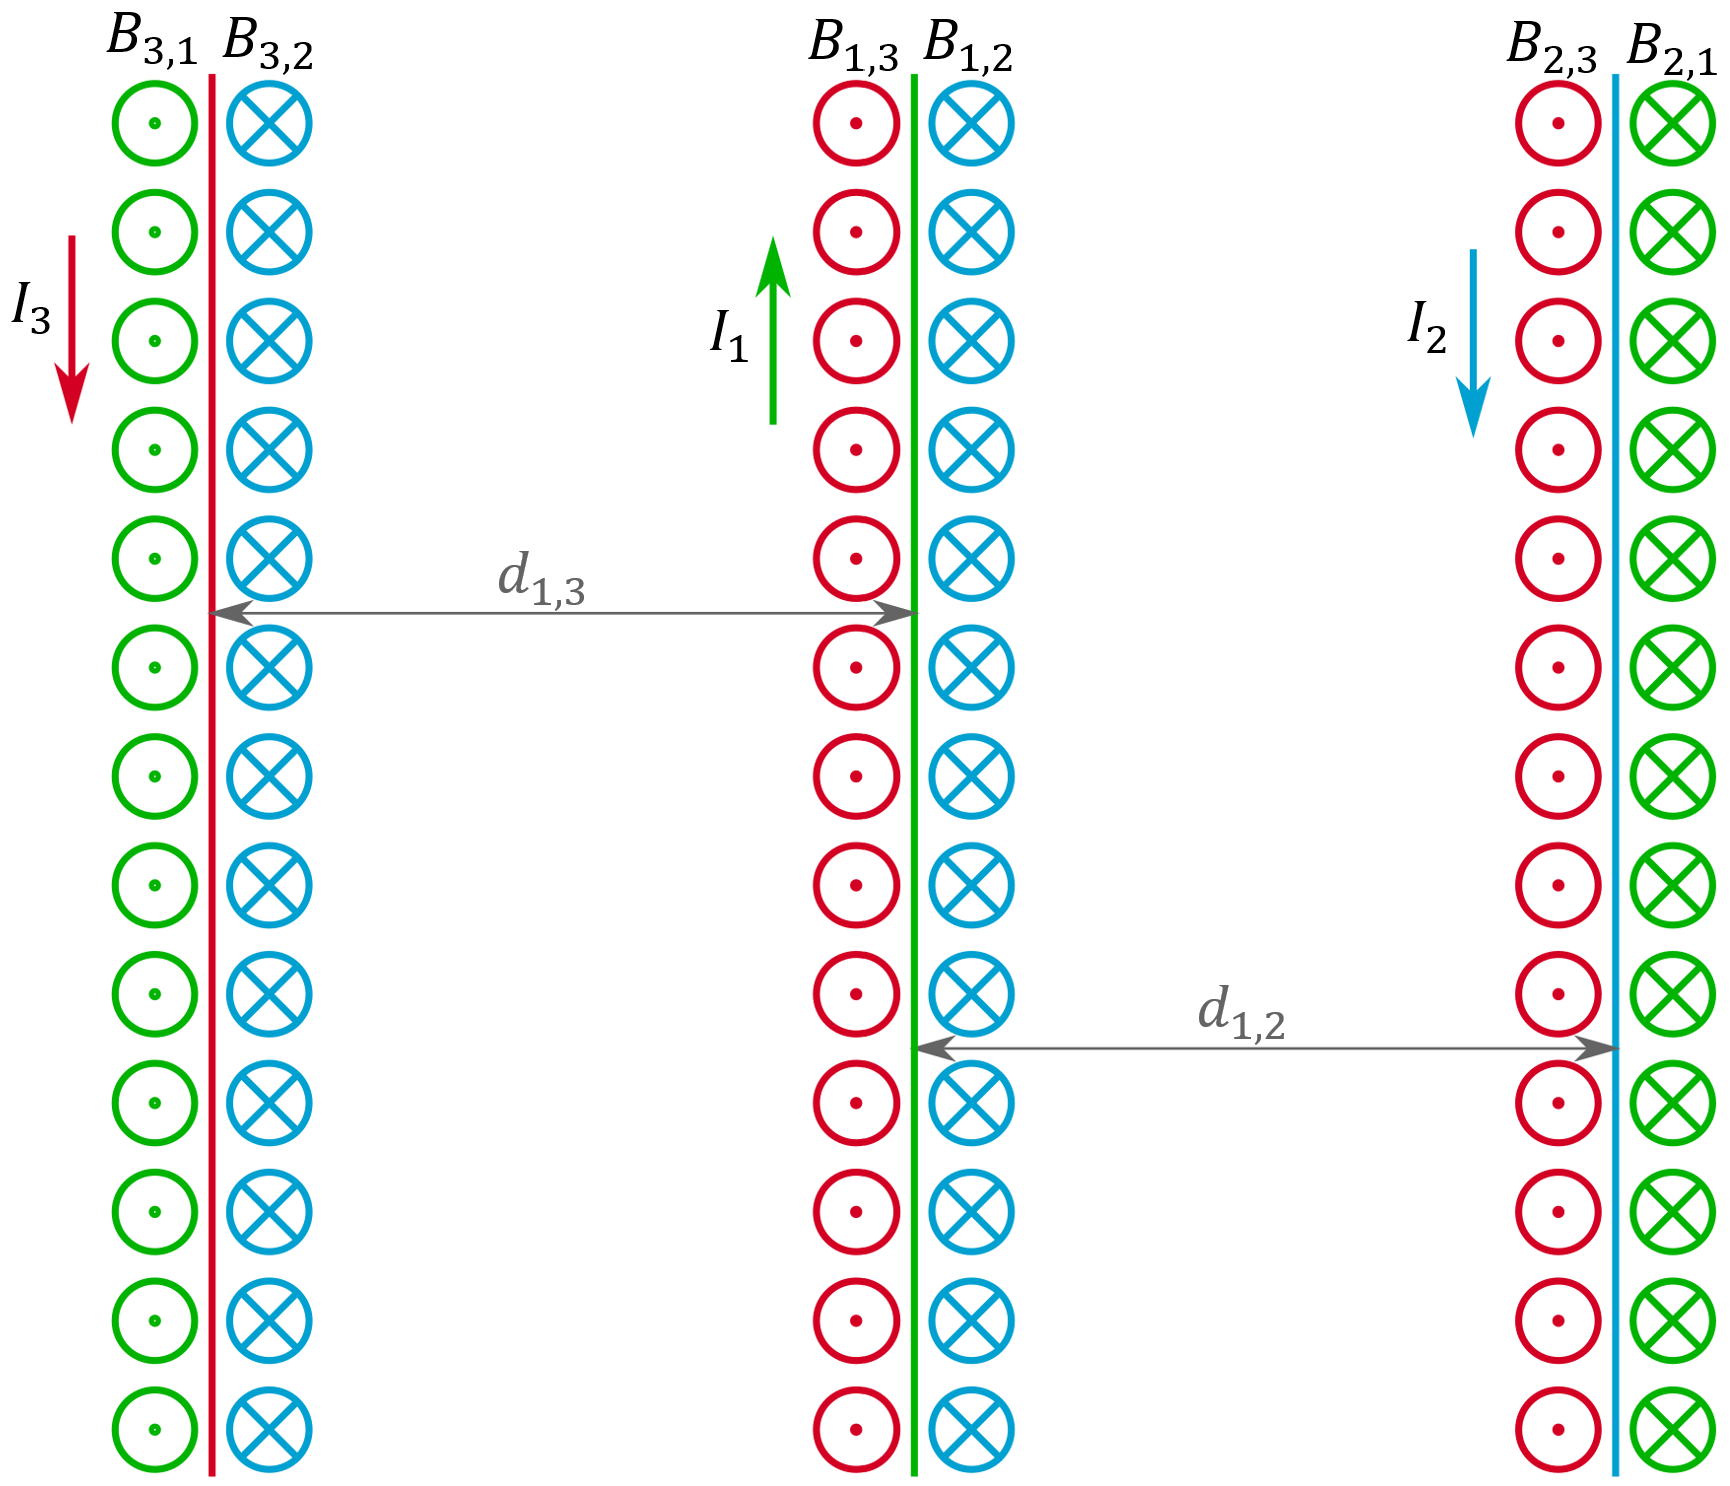
\includegraphics[width=8cm]{oz03/resources/oef-1-schets.png}
    
%     \textbf{Schets 3.1}
% \end{figure}

% \begin{enumerate}[(a)]
%     \item Ja het is mogelijk, er is 1 oplossing.
%     \item 
%         \begin{description}[labelwidth=1.5cm, leftmargin=!]
%             \item[Gevr. :]  $ d_{1,3} $; $ I_3 $;
%             \item[Opl. :]   Het totaal magnetisch veld in elke draad moet 0 zijn
            
%                             $ B_1 = 0 $
                            
%                             \hspace{-0.57cm} $ \Leftrightarrow -B_{1,2} + B_{1,3} = 0 $
                            
%                             \hspace{-0.57cm} $ \Leftrightarrow 
%                             -\dfrac{\mu_0 I_2}{2 d_{1,2}} + \dfrac{\mu_0 I_3}{2 d_{1,3}} = 0 $
                            
%                             \hspace{-0.57cm} $ \Leftrightarrow 
%                             -d_{1,3} I_2 + d_{1,2} I_3 = 0 $
                            
%                             \vspace{0.3cm}
                            
%                             $ B_2 = 0 $
                            
%                             \hspace{-0.57cm} $ \Leftrightarrow -B_{2,1} + B_{2,3} = 0 $
                            
%                             \hspace{-0.57cm} $ \Leftrightarrow 
%                             -\dfrac{\mu_0 I_1}{2 d_{1,2}} + \dfrac{\mu_0 I_3}{2 d_{2,3}} = 0 $
                            
%                             \hspace{-0.57cm} $ \Leftrightarrow 
%                             -d_{2,3} I_1 + d_{1,2} I_3 = 0 $
                            
%                             \vspace{0.3cm}
                            
%                             $ B_3 = 0 $
                            
%                             \hspace{-0.57cm} $ \Leftrightarrow B_{3,1} - B_{3,2} = 0 $
                            
%                             \hspace{-0.57cm} $ \Leftrightarrow 
%                             \dfrac{\mu_0 I_1}{2 d_{1,3}} - \dfrac{\mu_0 I_2}{2 d_{2,3}} = 0 $
                            
%                             \hspace{-0.57cm} $ \Leftrightarrow 
%                             d_{2,3} I_1 - d_{1,3} I_2 = 0 $
                            
%                             \hspace{-0.57cm} $ \Rightarrow 
%                             \left\{\begin{array}{l}
%                                 -d_{1,3} I_2 + d_{1,2} I_3 = 0 \\
%                                 -d_{2,3} I_1 + d_{1,2} I_3 = 0 \\
%                                 d_{2,3} I_1 - d_{1,3} I_2 = 0
%                             \end{array}\right. $
                            
%                             \hspace{-0.57cm} $ \Leftrightarrow 
%                             \left\{\begin{array}{l}
%                                 -d_{1,3} \cdot 4,00 + 20,0 \cdot I_3 = 0 \\
%                                 -(d_{1,3} + 20,0) \cdot 1,50 + 20,0 \cdot I_3 = 0 \\
%                                 (d_{1,3} + 20,0) \cdot 1,50 - d_{1,3} \cdot 4,00 = 0
%                             \end{array}\right. $
                            
%                             \hspace{-0.57cm} $ \Leftrightarrow 
%                             \left\{\begin{array}{l}
%                                 -d_{1,3} \cdot 4,00 + 20,0 \cdot I_3 = 0 \\
%                                 -(d_{1,3} + 20,0) \cdot 1,50 + 20,0 \cdot I_3 = 0 \\
%                                 -2,5 \cdot d_{1,3} = -30
%                             \end{array}\right. $
                            
%                             \hspace{-0.57cm} $ \Leftrightarrow 
%                             \left\{\begin{array}{l}
%                                 -d_{1,3} \cdot 4,00 + 20,0 \cdot I_3 = 0 \\
%                                 -(d_{1,3} + 20,0) 1,50 + 20,0 \cdot I_3 = 0 \\
%                                 d_{1,3} = 12,0 \textrm{ cm}
%                             \end{array}\right. $
                            
%                             \hspace{-0.57cm} $ \Leftrightarrow 
%                             \left\{\begin{array}{l}
%                                 -12,0 \cdot 4,00 + 20,0 \cdot I_3 = 0 \\
%                                 -(12,0 + 20,0) 1,50 + 20,0 \cdot  I_3 = 0 \\
%                                 d_{1,3} = 12,0 \textrm{ cm}
%                             \end{array}\right. $
                            
%                             \hspace{-0.57cm} $ \Leftrightarrow 
%                             \left\{\begin{array}{l}
%                                 I_3 = 2,40 \textrm{ A} \\
%                                 I_3 = 2,40 \textrm{ A (Uitgerekend ter controle)} \\
%                                 d_{1,3} = 12,0 \textrm{ cm}
%                             \end{array}\right. $
                            
%         \end{description}
% \end{enumerate}

% \vspace{1cm}